Dostává se Vám do ruky uživatelský manuál modelu \smod. Celý název modelu je: Simulační Model Povrchového Odtoku a Erozního Procesu. Tento model lze využít pro výpočet hydrologicko erozních procesů na jednotlivých pozemcích nebo na malých povodích. Výstupy z modelu jsou primárně určeny pro stanovení odtokových poměrů v ploše povodí a parametrů opatření pro snížení odtoku z povodí a erozního ohrožení zemědělské půdy. Model lze využít při navrhování komplexnějších soustav sběrných a odváděcích prvků nebo suchých nádrží a polderů. Jeho využití předpokládají jak současné metodiky, tak i technické normy a doporučené standardy.
Z hlediska kategorizace se jedná o fyzikálně založený plně distribuovaný dvourozměrný epizodní model. 
% 
Nově zavedené prostorové řešení (2D), které nahradilo dřívější profilovou verzi modelu, umožňuje komplexní řešení a náhled na celou řešenou lokalitu a přesnější popis zpravidla heterogenní morfologie zemského povrchu. 
% 
Přechod modelu na 2D řešení umožňuje zejména větší dostupnost potřebných dat a zvyšující se kapacita výpočetní techniky. 
% 
% Přesto, že dvourozměrné řešení je z hlediska vstupních dat a vnitřních procesů složitější, nicméně benefity distribuovaného řešení převažují. 
% Dostupnost vstupních dat v podrobném rozlišení se zlepšuje, stejně tak jako se zvyšuje výpočetní kapacita výpočetní techniky.
% 
% 
Vývoj modelu je podporován z veřejných prostředků a podílejí se na něm studenti a zaměstnanci Katedry hydromeliorací a krajinného inženýrství Fakulty stavební ČVUT v Praze.
Pro snazší orientaci je manuál rozdělen na dvou hlavních částí. 
% 
V první části jsou uvedeny zvolené výpočetní vztahy pro popis povrchového odtoku. 
% 
Druhá část je věnována popisu instalace a použití modelu v prostředí ArcGIS. Dále jsou zde podrobně popsána vstupní a výstupní data a stručně popsán tok programu. 
% Ve třetí části jsou ukázány výsledky z řečení konkrétní lokality.
Případné aktualizace, vzorová data, ukázky využití a další informace o modelu \smod jsou průběžně poskytovány na webových stránkách (\href{http://storm.fsv.cvut.cz/cinnost-katedry/volne-stazitelne-vysledky/smoderp/?lang=cz}{storm.fsv.cvut.cz/cinnost-katedry/volne-stazitelne-vysledky/smoderp/}).


\subsection*{Hydrologické modelování}\addcontentsline{toc}{subsection}{Hydrologické modelování}
Hydrologické modelování s využitím geografických informačních sytému (GIS) je oblast vyvíjející se od konce 70. let. Hydrologické modelu využívaly (a využívají) technologii operací s geodaty a databázemi, které GIS umožňuje. Přesto jsou některé topologické operace pro hydrologické modely specifické (např. definice rozvodnice povodí, lokalizace/odstranění bezodtokových míst)~\citep{devantier1993}. V zásadě se rozvíjeli modelu povrchového odtoku založené na pravidelném rastru, nepravidelné trojúhelníkové síťi (TIN) nebo na vrstevnisích (contour-based)~\citep{devantier1993}. Rovněž docházelo k vývoji celistvých~\footnote{povodí je rozděleno na sub-povodí která jsou řešena celistvě například metodou SCS křivek} nebo plně distribuovaných modelů~\citep{devantier1993}. S vývojem informační techniky docházelo k větší integraci GIS softwaru a hydrologických modelů. Na obrázku~\ref{fig:klasGISHyd} je ukázána klasifikace propojení GIS a hydrologických modelu na konci 90. let~\citep{sui1999}. Hydrologický model buďto pouze využívá některé funkcionality GIS softwaru (obrázek~\ref{fig:klasGISHyd}a). V opačném případě již vývojář GIS softwaru integruje do systému některé prvky hydrologických modelů (obrázek~\ref{fig:klasGISHyd}b). GIS software a hydrologické model si pouze vyměňují některá data (pomocí binárních nebo ascii souborů (obrázek~\ref{fig:klasGISHyd}c), nebo GIS software umožňuje ve svém prostření vložit uživatelem vytvořené skripty, která pak tvoří hydrologický model (obrázek~\ref{fig:klasGISHyd}b)\footnote{Toto je případ modelu SMODERP2D pokud je spouštěn v prostředí ArcGIS}~\citep{sui1999}. Autoři studie se k těmto postupů staví kriticky. Jejich základní výhradou je, že struktury GIS software vytvářejí bariery pro popis hydrologických dějů, které mají jistá specifika. Konceptualizace pomocí vrstev ať už rastrových  nebo vektorových nemusí vyjadřovat heterogenitu hydrologických dějů nebo užití stochastických modelů. GIS softwary často umožňují pouze limitovanou prací časové proměnlivými ději~\citep{sui1999}.

\begin{figure}
  \centering
  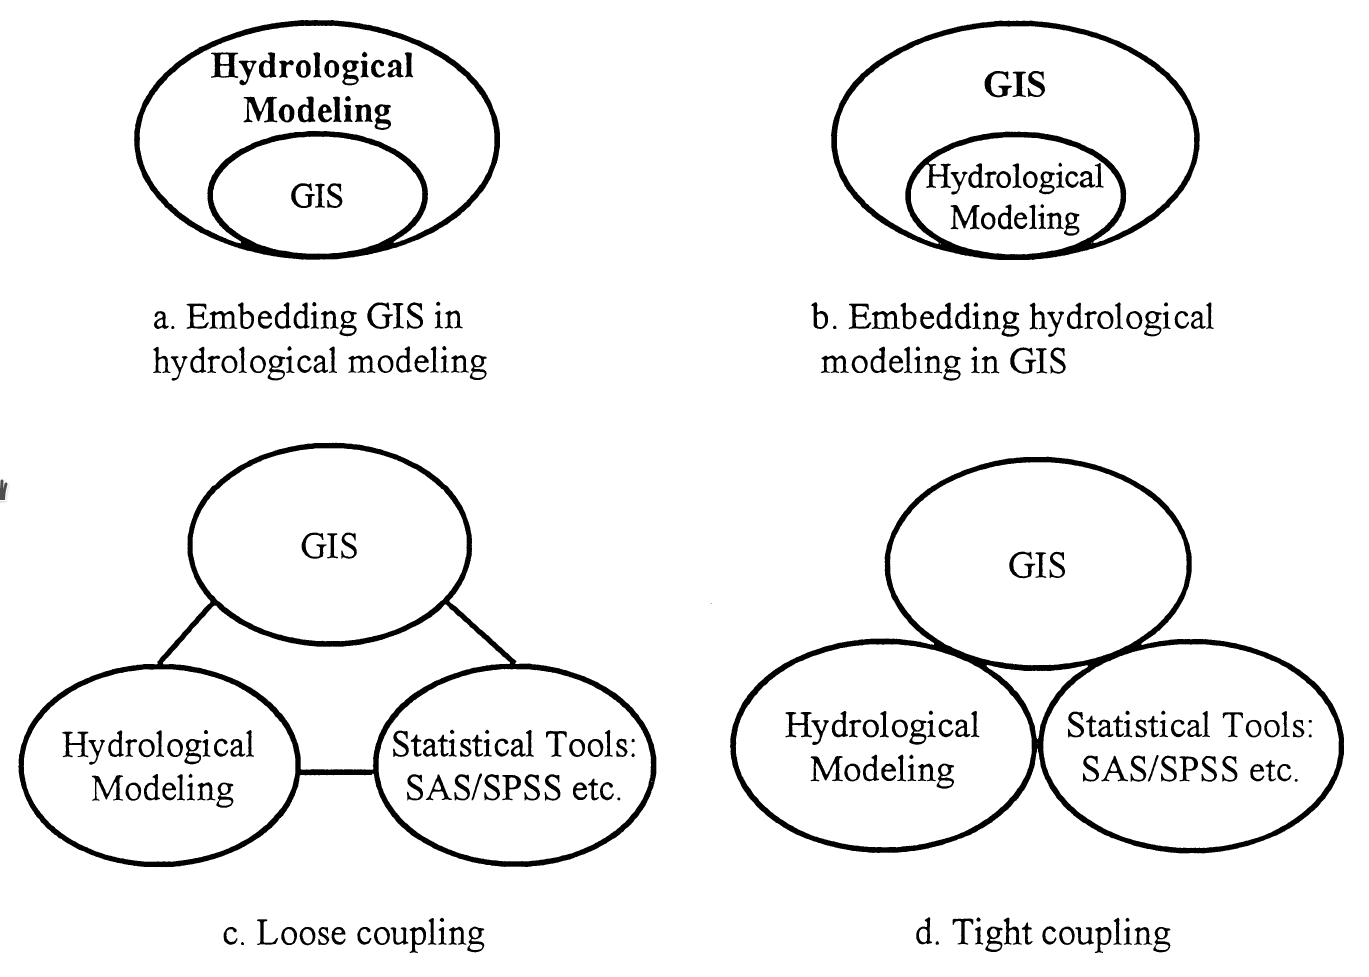
\includegraphics[width=0.75\linewidth]{./img/klasifikaceGISHyd.png}
  \caption{Klasifikace integrace hydrologických modelu podle~\cite{sui1999}}
  \label{fig:klasGISHyd}
\end{figure}

Při popisu povrchového odtoku se nejčastěji využívá jedno ze zjednodušení Saint-Venantových (SV) rovnic ať už kinematickou nebo difuzní. 
\pozn{Diffuzni vlna zjednodušuje SV rovnice tím, že zanedbava člen konvekčního zrychlení (setrvacnost) (Chaudhry, 1993). pochopit a doplnit}
Příklad řešení povrchového odtoku pomocí kinematickou například: \cite{taylor1974} nebo \cite{goodrich1991}. V případě druhé studie bylo 2D řešení kinematické vlny řešeno pro jednotlivé trojúhelníky TIN sítě. Celkový odtok byl pak výpočtem 1D routingem odtoku z jednotlivých trojúhelníků TIN sítě. Kinematická vlna pro řešení povrchového odtoku je implementována například v modelu HEC-1~\citep{macarthur1993}. Jako příklad řešení povrchového odtoku pomocí difuzní vlny může být například~\cite{julien1995}, kde byla rovněž implementována prostorově distribuovaná srážka vhodná pro řešení bleskových povodí v aridních oblastech. V \cite{jain2004} bylo směrování odtoku definované pomocí jednosměrného algoritmu D8, samotný byla ale řešen pomocé difuzní vlny. Jako příklady softwaru, kde byla využita difuzní vlna k řešení povrchového odtoku je například: SHE~\cite{abbott1986_1, abbott1986_2}, CAS2D~\cite{julien1995}, WEPP~\citep{flanagan2010} nebo SWAT ~\citep{USDA}. 

V literatuře lze rovněž najít kritéria na základě kterých lze určit vhodnost obou řešení. Využitelnost kinematické nebo difuzní vlny záleží na podmínkách daného řešeného území, počáteční podmínce nebo charakteristice srážky. Příkladem toho může být bezrozměrné číslo $\gamma$,které určí přesnost kinematické a difuzní vlny v porovnáním s dynamickou vlnou (přednější aproximace SV rovnic) v závislosti na počáteční podmínce, sklonu a drsnosti povrchu~\cite{singh1994}. Dalším příkladem může být kinematické číslo $K$, použité například v pro určení vhodnosti kinematické aproximace v úloze s proměnlivou srážkou~\citep{moramarco2002}. V některých případech jsou obě, kinematická i difuzní vlna, vhodnou aproximací pro řešení povrchového odtoku i na území povodí~\citep{Kazezyilmaz-Alhan2007}.

Obecné problémy v hydrologických modelech mohou nastat s nastavením časové a prostorové diskretizace.  U řešení povrchového odtoku byly zjištěny problémy s časovou diskretizací, kde docházelo k nestabilitám i při dodržení Courant–Friedrichs–Lewiho kritéria. To je způsobeno zejména malou hloubkou hladiny na povrchů vůči velikosti buňky rastru, drsnostnímu koeficientu nebo změně sklonu mezi sousedícími buňkamiA~\cite{zhang1989, esteves2000}. V \cite{molnar2000} byl studován vliv velikosti buňky rastru na výsledek modlu povrchového odtoku. Různá velikost buněk v rastru příliš neovlivňovala výsledné řešení pokud byla kalibrace provedena na rastru se stejně velkou buňkou. U řešení s větší buňkou bylo na povodí větší oblast, kde vznikl povrchový odtok a po kalibraci byla větší drsnost koryt hydrografické sítě.



\subsection*{Historie modelu}
Model je vyvíjen od konce osmdesátých let na KHMKI FSv ČVUT a od té doby byl několikrát modifikován. Jednotlivé verze jsou označeny, tak jak jsou označovány pro uživatele.

\paragraph*{Verze 04.89 - MS DOS – Programovací jazyk Fortran}

% První měření vedoucí ke stanovení odtokových parametrů na sklopném hydraulickém žlabu provedli pracovníci katedry hydromeliorací Fakulty stavební v Praze pod vedením M. Holého v roce 1984 (Holý, 1984). Výzkum byl prováděn na sklopném hydraulickém žlabu v laboratoři v Brně. Při různých sklonech dna žlabu a různých zeminách byly při zvolených průtocích vody měřeny výšky úrovně hladiny. Na základě těchto měření byl stanoven vztah pro výpočet průtoku na základě hloubky vody.

První verze modelu byla vyvinuta na ČVUT v roce 1989 pod vedením M. Holého. Byla napsána v programovacím jazyku FORTRAN. Zahrnovala v sobě procesy ovlivňující povrchový odtok a erozi. Submodel pro výpočet přípustné délky byl od submodelu pro výpočet odtokových charakteristik zcela oddělen a jednalo se spíše o dva nezávislé modely. Časový krok modelu byl zvolen v délce 0.2 minuty.

Před zadáním vstupních parametrů uživatel volil mezi submodelem 1 nebo submodelem 2. Zadávání probíhalo ve čtyřech krocích. V prvním kroku uživatel definoval morfologii svahu, kdy svah je definován dvojicí hodnot, první je vodorovná vzdálenost vrstevnic odečtená z mapy a druhou hodnotou je odlehlost (výšková vzdálenost) vrstevnic. Nevýhodou této verze modelu bylo, že odlehlost vrstevnic byla dána fixně a nebylo možné vkládat jakékoli jiné úseky než ty, které leží přesně mezi dvěma vrstevnicemi. To odpovídalo tehdejšímu způsobu získávání dat ručním odečítáním z tištěné mapy 1 : 10 000 nebo 1 : 5 000.

Ve druhém kroku uživatel na takto definovaných vzdálenostech vrstevnic volil půdní druh. Protože tehdejší možnosti výpočetní techniky byly limitované hardwarovými prostředky, byl počet takto zadaných úseků omezen na deset. V případě delších svahů, kde bylo více než deset vrstevnic, byl uživatel nucen některé části svahu spojovat do delších úseků. Tímto vyhlazením profilu docházelo k úpravě morfologie.

Ve třetím kroku byl uživatelem volen typ vegetace pro jednotlivé úseky. Úsek lze definovat jako homogenní celek, který má konstantní sklon, půdní druh a typ vegetace.

V posledním kroku uživatel zadával srážkové údaje, a to buď jako reálné srážky přímo změřené v terénu nebo návrhové srážky časově proměnné intenzity.

Doba vzniku modelu je již počítačovou historií, a tak i ovládání programu bylo poměrně náročné. Například vstupní parametry se musely při každém spuštění programu znovu zadávat, také neexistovala možnost vypočtené výsledky jakýmkoliv způsobem exportovat nebo ukládat. Používání modelu bylo tedy velmi komplikované. Proto byla vytvořena jeho aktualizovaná verze.

\paragraph*{Verze IV. I/11 – 96 - MS DOS – Programovací jazyk Fortran}

V devadesátých letech byla vytvořena druhá verze modelu. V ní se podařilo odstranit několik základních nedostatků z předchozí verze. Již bylo možné zpětně editovat dříve vypočtené pozemky. Také bylo možné ukládat a tisknout získané výpočty. Úpravy se však týkaly jen prostředí a vedly k usnadnění práce uživatele. Při této aktualizaci nedošlo k žádné úpravě vnitřních výpočetních vztahů.


\subsection*{SMODERP1D}\addcontentsline{toc}{subsection}{Historie modelu - SMODERP1D}

SMODERP1D je starší verze modelu SMODERP2D. Model byl určen ke stanovení charakteristik plošného odtoku v 1D profilech řešeného svahu a stanovené nejdelší bezpečné odtokové dráhy (Obrázek~\ref{fig:smod1d}).

\begin{figure}
  \centering
  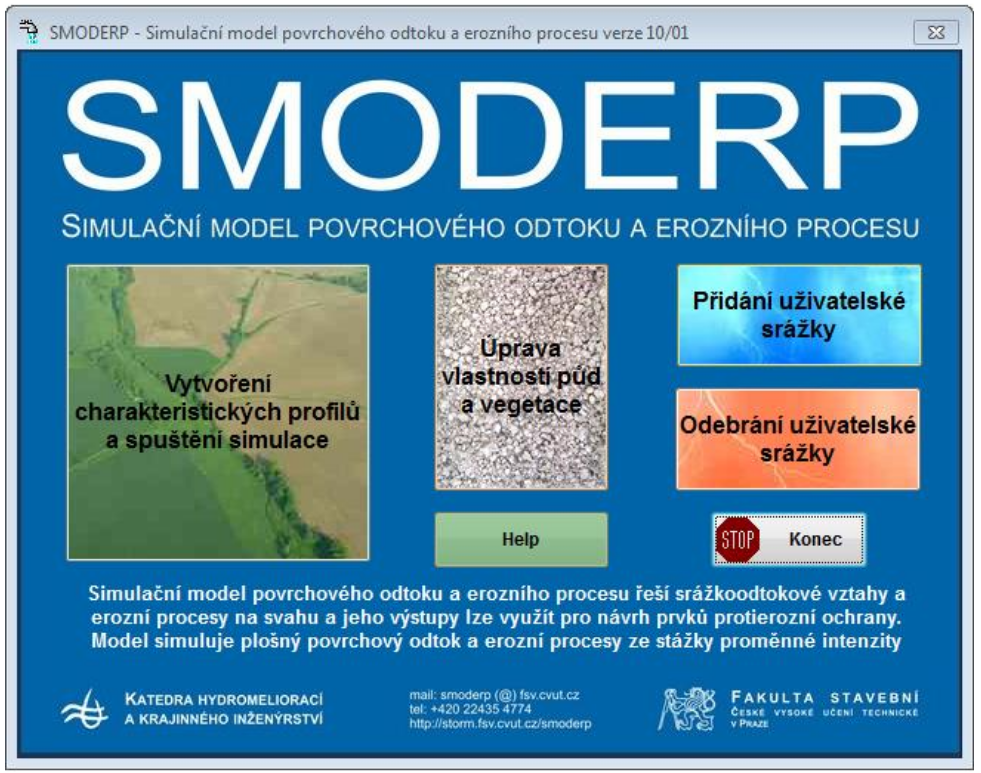
\includegraphics[width=0.75\linewidth]{./img/smo1d.png}
    \caption{Úvodní obrazovka modelu SMODERP1D}
  \label{fig:smod1d}
\end{figure}


\paragraph*{Programovací jazyk Visual Basic (konečná verze 5.01)}

S příchodem nového prostředí Windows již nebylo možné předchozí DOS verzi spustit, proto byla od roku 1999 vyvíjena další generace modelu. Hlavní změnou byl posun od prostředí MS-DOS k uživatelsky přístupnějšímu prostředí Windows. Uživatelsky byl tento směr krokem vpřed. Způsob zadávání vycházel z jedné vstupní obrazovky, kde uživatel zvolil zadávání svahů, srážek, případně vegetace. Dalším kladem byla možnost zadat a vypočítat několik svahů najednou. Všechny tyto úpravy vedly ke zjednodušení a zrychlení práce. Postupně vzniklo celkem šest verzí modelu, které se částečně lišily vzhledem a dostupností obou submodelů.

Úpravy se týkaly především uživatelského rozhraní, výpočtové části se změny týkaly jen minimálně. Některé z  nedostatků byly postupně odstraňovány, šlo většinou o úpravu drobných chyb a případně o zjednodušení práce pro uživatele. Výsledkem spojení verze pro MS-DOS, programově vycházející z jazyka FORTRAN, a Visual Basicu byla občasná nestabilita programu, která se projevuje zhroucením výpočtu (například při větším počtu úseků, při krátkých úsecích apod.).

V roce 1999 vznikla první verze s označením 1.01, v  níž byla funkční pouze simulace erozní ohroženosti a stanovení přípustných délek. Tato verze byla aktualizována v roce 2001 pod označením verze 2.20 a byla dlouhou dobu ke stažení z webových stránek FSv ČVUT v Praze (FSv – KHMKI, 2010). Především šlo o vylepšení uživatelského rozhraní. V roce 2001 byla také vytvořena zkušební verze 3.55, ve které byl zahrnut kromě simulace erozní ohroženosti i výpočet odtokových charakteristik. Tato verze byla v roce 2003 aktualizována zcela funkční verzí 4.01. Poslední verzí, která přímo vychází a navazuje na předchozí verze, má označení 5.1 a vznikla v roce 2010. V této verzi je aktualizován vztah pro výpočet průtoku a do této verze je možné doplnit rekalibrované odtokové parametry. 

\paragraph*{Programovací jazyk Visual Fox Pro (Verze 10.01)}

Od roku 2006 byla vytvářena nová verze modelu SMODERP, která zahrnuje nové poznatky v nově napsaném zdrojovým kódu. V této verzi jsou zahrnuty nově stanovené rekalibrované odtokové parametry, stanovené na základě řady dalších měření na sklopném hydraulickém žlabu ve vodohospodářské  laboratoři Fakulty stavební ČVUT v Praze. Tato verze navazuje na předchozí verze použitím základních vztahů.  

